\subsection{Utility classes}

\begin{figure}[h]
	\centering
	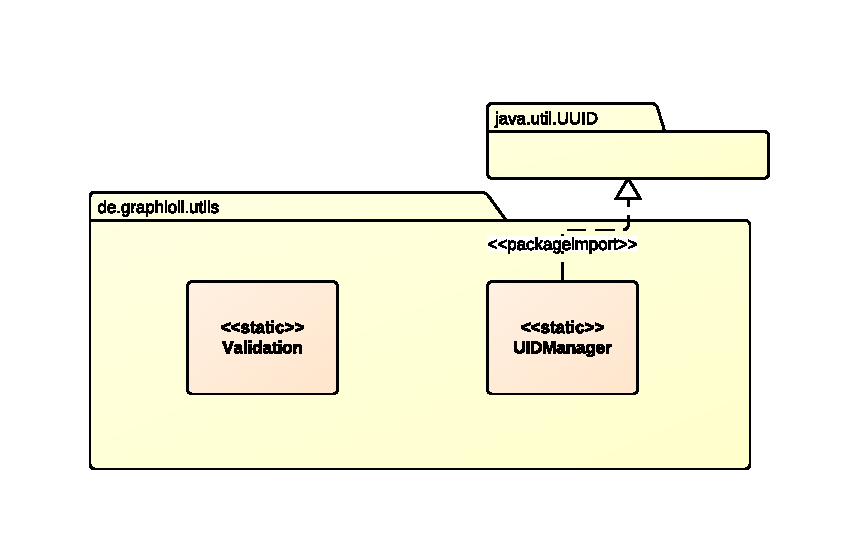
\includegraphics[page=1,width=\textwidth,keepaspectratio]{utilsClassDiagram.pdf}
	\caption{Utility class diagram.}
	\label{img:utilsClassDiagram}
\end{figure}
\pagebreak

% Validation
\static{Validation}{validation}
This class provides \gls{static-method}s for checking the validity of given values. \\

\vspace{.5cm}
\hrule

\paragraph*{Method Summary}
\paragraph*{}
\begin{longtable}{Lp{10cm}}
	\startmethodtable
	\method{public static boolean}{isValidFile(File file)}{validation:isvalidfile} \\
	& Checks if the specified file is valid. \\
	\method{public static boolean}{isValidPlayerName(String name)}{validation:isvalidplayername} \\
	& Checks if the specified string is a valid \ref{cls:player} name. \\
	\hline
\end{longtable}

% UIDManager
\static{UIDManager}{uidmanager}
This class is responsible for creating unique \glspl{ID} by using the \texttt{java.util.UUID} package.  \\

\vspace{.5cm}
\hrule

\paragraph*{Method Summary}
\paragraph*{}
\begin{longtable}{Lp{10cm}}
	\startmethodtable
	\method{public static UUID}{generateUniqueID()}{uidmanager:generateuniqueid} \\
	& Generates a unique \gls{ID}. \\
	\method{private static boolean}{isUnique(UUID uuid)}{uidmanager:isunique} \\
	& Helper method, which ensures that a generated \gls{ID} is really unique. \\
	\hline
\end{longtable}